\documentclass{standalone}
\usepackage{tikz}
\begin{document}
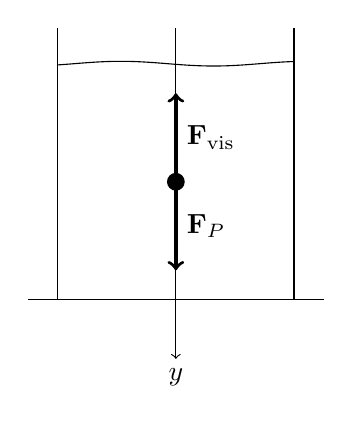
\begin{tikzpicture}[scale=1.5]
    \draw[-](-0.25,0)--(2.25,0);
    \draw[-](0,0)--(0,2.3);
    \draw[-](2,0)--(2,2.3);

    \filldraw[black](1,1)circle(2pt);
    \draw[->,very thick](1,1)--(1,0.25)node[midway, right]{$\mathbf{F}_P$};
    \draw[->,very thick](1,1)--(1,1.75)node[midway, right]{$\mathbf{F}_\mathrm{vis}$};
    \draw[->](1,2.3)--(1,-0.5)node[below]{$y$};

    \draw[-] plot[smooth, domain=0:2] (\x, {2+0.02*sin(4*(\x+3) r)});
\end{tikzpicture}
\end{document}